\documentclass[12pt, a4paper]{report}
\usepackage[top=1.0in, bottom=1.0in, left=0.8in, right=0.8in]{geometry}
\usepackage{graphicx}
\usepackage{amsmath}
\usepackage{listings}
\usepackage{fancyvrb}

 	
\title{\textbf{EE2703 : Applied Programming Lab \\ Endsem \\ Antenna currents in a half-wave dipole antenna}} 
\author{Aditya Nanda Kishore\\ EE20B062} 

\date{\today} % Date for the report

	
\begin{document}
		
\maketitle
\section*{Introduction}
We are given a half-wave dipole antenna and it's parameters.Our aim is to find the antenna currents in a half-wave dipole antenna. The parameters go like this 

\begin{itemize}
	\item Half-length $l= 0.5 m$
	\item Number of sections in each half section N = 4 and is changed to 100 later for better accuracy
	\item Feeding current $I_m = 1 A$
	\item Radius of wire $a= 0.05 m$
	\item c = $2.9979 * 10^8 m/s$ and $\mu_0 = 4\pi*10^{-7}$ 
\end{itemize}

It is known that 

\begin{equation*}
I(z) =  \left\{
        \begin{array}{ll}
            I_msin(k(l-z)) & \quad 0 \leq z \leq l  \\
            I_msin(k(l+z))& \quad -l \leq z \leq 0
        \end{array}
    \right.
\end{equation*}

The problem is to determine if this is valid.


\section*{Setting up required variables and vectors}
I called a few dependent parameters like $dz$ and wave number
\begin{itemize}
	\item $dz = l/N$
	\item $k = 2\pi/4l = \pi$
\end{itemize}

A z vector with all the z co-ordinates of the samples is created.The current vector has $2N+1$ elements corresponding to current at each one of the above z and three of them are known. $J[0] = J[-1] = 0$ and $J[N]=I_m$. So we will define another vector J with only the unknowns and another vector u is created with the co-ordinates of the unknowns.
\begin{equation*}
J = 
  \begin{pmatrix}
    J_1\\
       J_2 \\
           .\\
           .\\
           J_{N-1}\\
           J_{N+1}\\
           .\\
           .\\
           J_{2N-2}\\
           J_{2N-1}\\
  \end{pmatrix}
 u= 
  \begin{pmatrix}
    z_1\\
       z_2 \\
           .\\
           .\\
           z_{N-1}\\
           z_{N+1}\\
           .\\
           .\\
           z_{2N-2}\\
           z_{2N-1}\\
  \end{pmatrix}
\end{equation*}

\section*{Calculation of Magnetic Field}
\subsection*{Ampere's Law}
From Ampere’s Law, we have for $H_\phi(z,r=a)$

\begin{equation*}
2\pi a H_\phi(z_i) = J_i
\end{equation*}
Matrix form of the equation is(We are writing the equations only for unknowns)

\begin{figure}[!tbh]
   	\centering
   	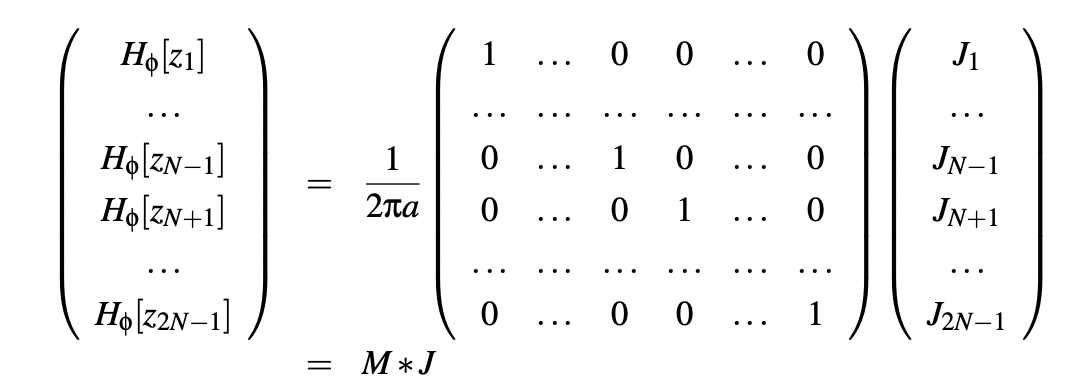
\includegraphics[scale=0.7]{A.png}
 \end{figure} 
 \vspace{0.5cm}
We have to take care that order of M is 2N-2 by 2N-2.
\subsection*{Vector Potential}
Vector potential along the circumference by currents at different parts of the antenna is given by
\begin{equation*}
\vec{A}(r,z) = \frac{\mu_0}{4\pi} \int_z  \frac{I(z')\hat{z} e^{-jkR} dz'_j}{R}
\end{equation*}
 
 where $\vec{R} = \vec{r} - \vec{r'} = r\hat{r} + (z-z')\hat{z}$ and $\vec{r'} = z'\vec{z'}$  is a point on the wire. Now, this integral can be reduced to a sum
 
\begin{equation*}
A_{z,i} = \frac{\mu_0}{4\pi}\sum_{j} ^{} \frac{I_je^{-jkR_{ij}}dz'_{ij}}{R_{ij}}
\end{equation*}

\begin{equation*}
A_{z,i} =\sum_{j} ^{} I_j (  \frac{\mu_0}{4\pi} \frac{I_je^{-jkR_{ij}}dz'_{ij}}{R_{ij}})
\end{equation*}

\begin{equation*}
A_{z,i} =\sum_{j} ^{} I_j P_{ij} + P_BI_N
\end{equation*}


where  
\large
$P = \frac{\mu_0}{4\pi}    \frac{e^{-jkR}dz'_{ij}}{R}$ and $P_B = \frac{\mu_0}{4\pi}    \frac{e^{-jkR_{iN}}dz'_{ij}}{R_{iN}}$
\newpage
\normalsize

So, we have to build R matrices first then we can build P matrices.
For building R matrix, I defined a R generator function that returns a matrix whose each row represents distance of the point we are interested in from every sampled point in z-axis. It can be written as 

\newline
$R_{ij}$ = (distance of point on circumference from z in x - direction) + j(distance of point on circumference from z in y - direction)

\newline
But distance of point on circumference from z in x - direction = radius = a

\newline
$R_{ij}$ = a + j(distance of point on circumference from z in y - direction)

So R generator function can have 2 arguments for real part and imaginary part, r and z respectively and the distances in y- direction can be obtained by subtracting the outputs of the meshgrid of z,z.For example let's take a simple z and r to understand this. let $z = [-2,-1,0,1,2]$ 
Meshgridding z by itself  will produce the outputs
\begin{equation*}
z_1 = 
  \begin{pmatrix}
    -2 &-1& 0 &1 &2\\
      -2 &-1& 0 &1 &2\\
        -2 &-1& 0 &1 &2\\
      -2 &-1& 0 &1 &2\\
          -2 &-1& 0 &1 &2\\
  \end{pmatrix}
 z_2= 
  \begin{pmatrix}
  -2& -2& -2 &-2& -2\\
  -1& -1& -1 &-1 &-1\\
  0& 0 &0 &0& 0\\
  1 &1& 1& 1 &1\\
  2& 2 &2 &2 &2\\
    \end{pmatrix}


\end{equation*}
\begin{equation*}
z_1-z_2=
  \begin{pmatrix}
  0& 1& 2 &3& 4\\
  -1& 0& 1 &2 &3\\
  -2& -1 &0 &1& 2\\
  -3&-2& -1& 0 &1\\
  -4& -3 &-2 &-1 &0\\
    \end{pmatrix}

 \end{equation*}
 
 Here if we clearly observe every row in the previous matrix is the successive distance of a point on the circumference from all points in z-axis along y-direction.
 


 So, We can set this up as imaginary part of the matrix and add $a$ as real part and  calculate the distance matrix, R successfully.
 For setting up real matrix we can use \textbf{a*np.ones}.
 
 \newline
So For \textbf{$R_z$} inputs would be \textbf{real matrix of order 2N+1 and z}. For \textbf{$R_u$} inputs would be \textbf{real matrix of order 2N-2 and u.}
\begin{equation*}
R_z= 
  \begin{pmatrix}
    a&a& .&. &a\\
       a&a& .&. &a\\
        . &.& . &. &.\\
         . &.& . &. &.\\
              a&a& .&. &a\\
  \end{pmatrix}
 +j
  \begin{pmatrix}
  z_{00}& z_{01}& . &.& z_{0(2N)}\\
  z_{10}& z_{11}& . &.& z_{1(2N)}\\
  .& . &. &.& .\\
  . &.& .& . &.\\
 z_{(2N)(0)}& z_{(2N)(1)}& . &.& z_{(2N)(2N)}\\

    \end{pmatrix}


\end{equation*}

\begin{equation*}
R_u= 
  \begin{pmatrix}
    a&a& .&. &a\\
       a&a& .&. &a\\
        . &.& . &. &.\\
         . &.& . &. &.\\
              a&a& .&. &a\\
  \end{pmatrix}
 +j
  \begin{pmatrix}
  z_{00}& z_{01}& . &.& z_{0(2N-3)}\\
  z_{10}& z_{11}& . &.& z_{1(2N-3)}\\
  .& . &. &.& .\\
  . &.& .& . &.\\
 z_{(2N-3)(0)}& z_{(2N-3)(1)}& . &.& z_{(2N-3)(2N-3)}\\

    \end{pmatrix}


\end{equation*}
 



Now For $P_B$ we might want Rz[N], but without those three known distances.We have to eliminate those and then substitute the newly formed list in the above $P_B$ expression.

 \vspace{1cm}

After using the above expression of Vector Potential to calculate H we would get something like this,


 \begin{equation*}
H_\phi(r,z_i) = \sum_{j} ^{} P_{ij} \frac{r}{\mu_0}(  \frac{jk}{R_{ij}} + \frac{1}{R_{ij}^2} )I_j + P_B\frac{r}{\mu_0}(  \frac{jk}{R_{iN}} + \frac{1}{R_{iN}^2} )I_m
 \end{equation*}
 
 
 \begin{equation*}
H_\phi(r,z_i) = \sum_{j} ^{} Q_{ij} I_j + Q_BI_m
 \end{equation*}
 
 So, We can write code for Q, $Q_B$
 
 After that, we can equate this equation to M*J and rearrange terms to get J.We can later convert that to a list and append the known terms J[0],J[N],J[2N] to the list, which would complete the function. Plotting that I got something like this for N=4 and N= 100
 \begin{equation*}
 J = I_m(M-Q)^{-1}Q_b
 \end{equation*}
 \newline

\begin{figure}[!tbh]
   	\centering
   	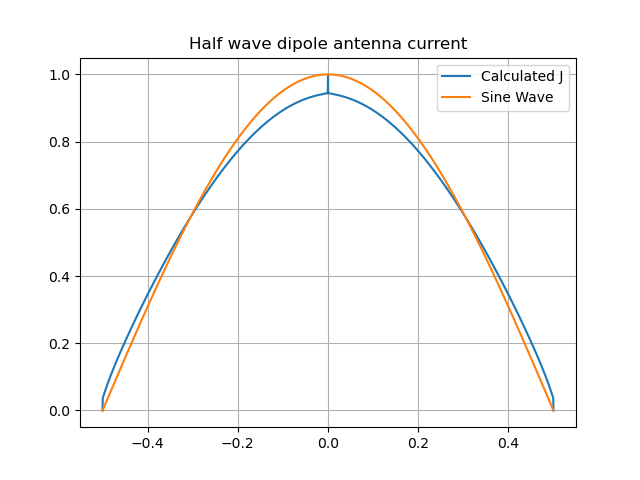
\includegraphics[scale=0.7]{Q5.png}
	\caption{Current plot for N = 4}
 \end{figure} 
 
 \begin{figure}[!tbh]
   	\centering
   	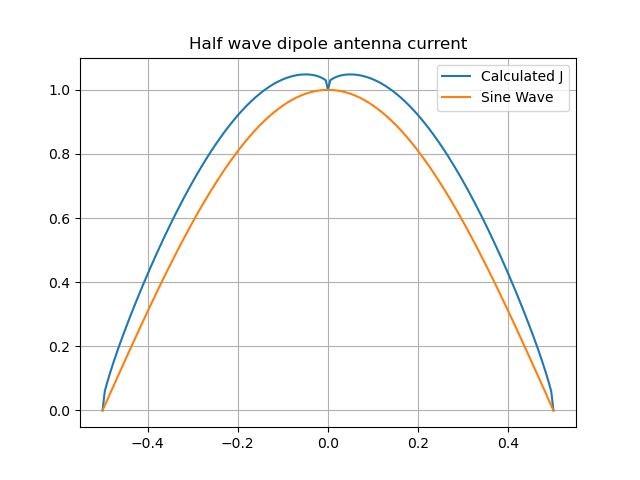
\includegraphics[scale=0.7]{Q5b.png}
	\caption{Current plot for N = 100}
 \end{figure} 
 \newpage
 Clearly, There is some discrepancy from the actual current here.It's because of the error in digitisation during sampling. Error must decrease if we increase N. But still, even for some larger N there was discrepancy.
  \section*{Matrices for N=4}
  
   The $M$ matrix is 
\begin{equation*}
\begin{pmatrix}
15.92 & 0.0 & 0.0 & 0.0 & 0.0 & 0.0\\
0.0 & 15.92 & 0.0 & 0.0 & 0.0 & 0.0\\
0.0 & 0.0 & 15.92 & 0.0 & 0.0 & 0.0\\
0.0 & 0.0 & 0.0 & 15.92 & 0.0 & 0.0\\
0.0 & 0.0 & 0.0 & 0.0 & 15.92 & 0.0\\
0.0 & 0.0 & 0.0 & 0.0 & 0.0 & 15.92\\
\end{pmatrix}
\end{equation*}
\vspace{0.5cm}
 
 The $R_z$ matrix is 
\begin{equation*}
    \begin{pmatrix}
0.13 & 0.01 & 0.13 & 0.25 & 0.38 & 0.5 & 0.63 & 0.75 & 0.88\\
0.25 & 0.13 & 0.01 & 0.13 & 0.25 & 0.38 & 0.5 & 0.63 & 0.75\\
0.38 & 0.25 & 0.13 & 0.01 & 0.13 & 0.25 & 0.38 & 0.5 & 0.63\\
0.63 & 0.5 & 0.38 & 0.25 & 0.13 & 0.01 & 0.13 & 0.25 & 0.38\\
0.75 & 0.63 & 0.5 & 0.38 & 0.25 & 0.13 & 0.01 & 0.13 & 0.25\\
0.88 & 0.75 & 0.63 & 0.5 & 0.38 & 0.25 & 0.13 & 0.01 & 0.13\\
\end{pmatrix}
\end{equation*}
\vspace{0.5cm}

 The $R_u$ matrix is 
\begin{equation*}
    \begin{pmatrix}
0.01 & 0.13 & 0.25 & 0.5 & 0.63 & 0.75\\
0.13 & 0.01 & 0.13 & 0.38 & 0.5 & 0.63\\
0.25 & 0.13 & 0.01 & 0.25 & 0.38 & 0.5\\
0.5 & 0.38 & 0.25 & 0.01 & 0.13 & 0.25\\
0.63 & 0.5 & 0.38 & 0.13 & 0.01 & 0.13\\
0.75 & 0.63 & 0.5 & 0.25 & 0.13 & 0.01\\
\end{pmatrix}
\end{equation*} 
\vspace{0.5cm}

The $P$ matrix is
\small
\begin{equation*}
    \begin{pmatrix}
(124.94-3.93j) & (9.2-3.83j) & (3.53-3.53j) & (-0-2.5j) & (-0.77-1.85j) & (-1.18-1.18j)\\
(9.2-3.83j) & (124.94-3.93j) & (9.2-3.83j) & (1.27-3.08j) & (-0-2.5j) & (-0.77-1.85j)\\
(3.53-3.53j) & (9.2-3.83j) & (124.94-3.93j) & (3.53-3.53j) & (1.27-3.08j) & (-0-2.5j)\\
(-0-2.5j) & (1.27-3.08j) & (3.53-3.53j) & (124.94-3.93j) & (9.2-3.83j) & (3.53-3.53j)\\
(-0.77-1.85j) & (-0-2.5j) & (1.27-3.08j) & (9.2-3.83j) & (124.94-3.93j) & (9.2-3.83j)\\
(-1.18-1.18j) & (-0.77-1.85j) & (-0-2.5j) & (3.53-3.53j) & (9.2-3.83j) & (124.94-3.93j)\\
\end{pmatrix}
\end{equation*}
\vspace{0.5cm}
\normalsize

The $P_b$ matrix is
\begin{equation*}
 \begin{pmatrix}
(1.27-3.08j) & (3.53-3.53j) & (9.2-3.83j) & (9.2-3.83j) & (3.53-3.53j) & (1.27-3.08j)\\
\end{pmatrix}
\end{equation*}
\vspace{0.5cm}
  
 The $Q$ matrix is
 \footnotesize
 \begin{equation*}
    \begin{pmatrix}
(99.521-0.001j) & (0.054-0.001j) & (0.008-0.001j) & (0.001-0.001j) & (0.001-0.001j) & -0.001j\\
(0.054-0.001j) & (99.521-0.001j) & (0.054-0.001j) & (0.003-0.001j) & (0.001-0.001j) & (0.001-0.001j)\\
(0.008-0.001j) & (0.054-0.001j) & (99.521-0.001j) & (0.008-0.001j) & (0.003-0.001j) & (0.001-0.001j)\\
(0.001-0.001j) & (0.003-0.001j) & (0.008-0.001j) & (99.521-0.001j) & (0.054-0.001j) & (0.008-0.001j)\\
(0.001-0.001j) & (0.001-0.001j) & (0.003-0.001j) & (0.054-0.001j) & (99.521-0.001j) & (0.054-0.001j)\\
-0.001j & (0.001-0.001j) & (0.001-0.001j) & (0.008-0.001j) & (0.054-0.001j) & (99.521-0.001j)\\
\end{pmatrix}
\end{equation*}
\vspace{0.5cm}
  
 \normalsize
 The $Qb$ matrix is
 \footnotesize
 \begin{equation*}
   \begin{pmatrix}
(0.003-0.001j) & (0.008-0.001j) & (0.054-0.001j) & (0.054-0.001j) & (0.008-0.001j) & (0.003-0.001j)\\
\end{pmatrix}
\end{equation*}
\vspace{0.5cm}
  
  \normalsize
  The I matrix is
   \begin{equation*}
   \begin{pmatrix}
0j & 0j & 0j & 0j & (1+0j) & 0j & 0j & 0j & 0j\\
\end{pmatrix}
\end{equation*}

\section*{Pseudocode}
\subsection*{Part 1}
\begin{Verbatim}
1.Define the variables and vectors I,J,u,z
2.Create the function M_generator(n,a) which returns identity matrix*(1/(2*pi*a)). 
3.Multiply Matrices M and J to get H.
\end{Verbatim}
\subsection*{Part 2}
\begin{Verbatim}
1.func R_generator(r,z):
	Create z1, z2  which are outputs of meshgrid(z,z)
	z = j*(z1-z2)
	Add r and z
	return Matrix with absolute value of the previous sum
2.Define rz and ru which contain 'a' as every element and have order of 2N+1 and 2N-2 
respectively
3.Apply R_generator on rz,z.Name it Rz
4.Apply R_generator on ru,u.Name it Ru
5.Create a new array with Rz[N]'s elements without the 0th, Nth, 2Nth elements.
\end{Verbatim}

\subsection*{Part 3}
\begin{Verbatim}
 1.Define P and Pb from R and Rb
 2.Define Q and Qb as given from P, Pb, Ru, Rz
 3.Find J from the equation given
 4.Append J with the known values J[0],J[N],J[2N]
 5.Plot J vs z.Compare with sinusoidal J.
 \end{Verbatim}


 
 
  \section*{Conclusions}
  \begin{itemize}
  \item In a Half-wave dipole Antenna, It's a fair assumption to assume that currents will be travelling in a half sinusoidal wave.
  \item Matrices and it's operations is a powerful and effective tool to find solutions when we are calculating any set of solutions with variables following a certain set of equations. 
  \item There are discrepancies in the current from the sinusoid because of the error in digitisation and the assumptions used while calculating the current theoretically.
  \end{itemize}
 

\end{document}